\documentclass[11pt]{beamer}
\usetheme{Madrid}
\usepackage[utf8]{inputenc}
\usepackage{listings}
\usepackage{tikz}
\usepackage{tkz-euclide}
\usepackage{amsmath}
\usepackage{amsfonts}
\usepackage{amssymb}
\usepackage{graphicx}
\lstset{
%language=C,
frame=single, 
breaklines=true,
columns=fullflexible
}
\setbeamercovered{transparent} 
\setbeamertemplate{navigation symbols}{} 
%\logo{} 

%\date{} 
%\subject{} 


\title{ASSIGNMENT 1}
\author{by Mohit Singh}
\institute{IIEST, Shibpur} 
\centering
\date{21 May 2020}

\begin{document}

\maketitle
\begin{frame}{PROBLEM}
\begin{block}{Exercise 8.1, Q36}
The side AB and BC and median AM of one triangle ABC are respectively equal to sides PQ and QR and median PN of triangle PQR. Show that:
\newline
\newline
{1)$\triangle  ABM  \cong   \triangle  PQN $}
\newline
{2) $\triangle  ABC  \cong   \triangle  PQR $}
\end{block}

\end{frame}

\begin{frame}[containsverbatim]{CODES}
Download the python code from
\begin{lstlisting}
./codes/triangle_python.py
\end{lstlisting}
and latex code from
\begin{lstlisting}
./fig/triangle_fig.tex
\end{lstlisting}
\end{frame}

\begin{frame}{FIGURES}
\begin{figure}
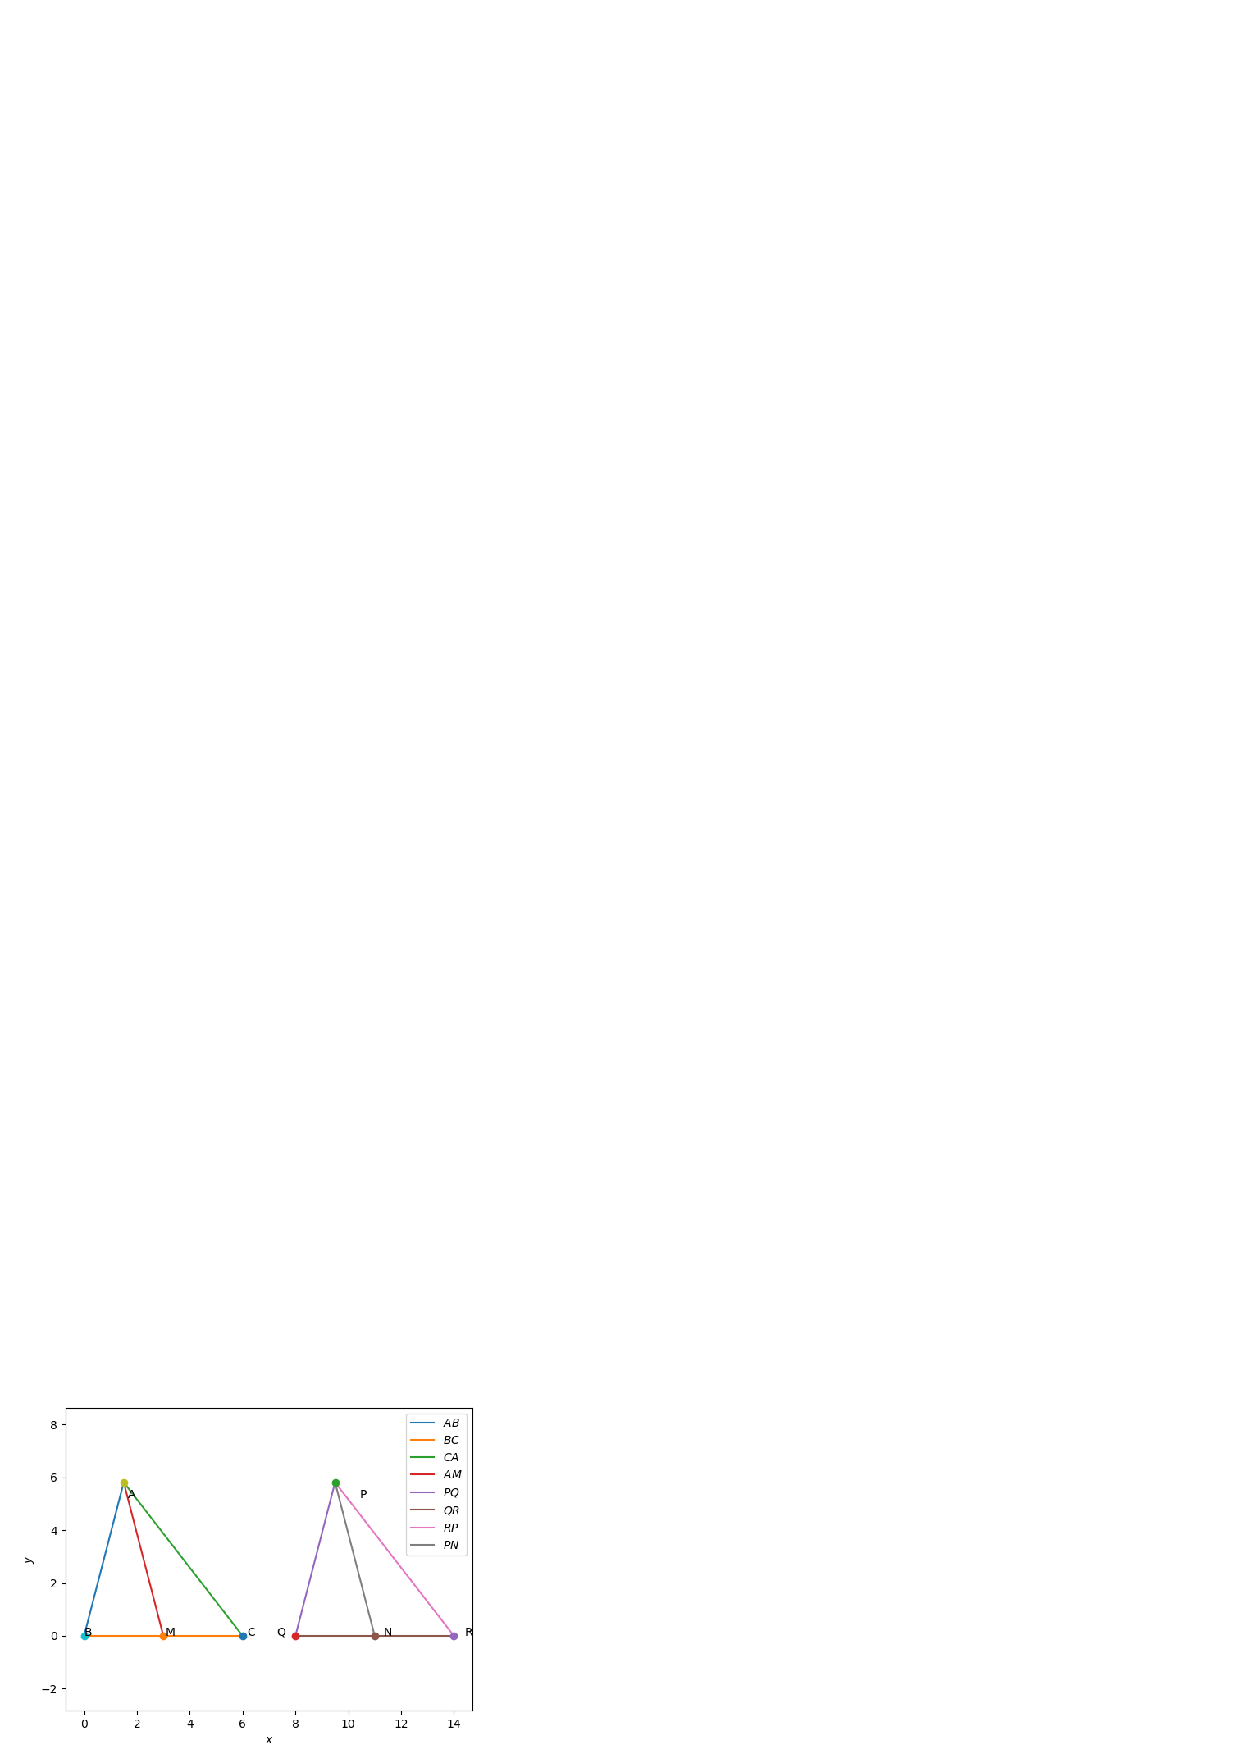
\includegraphics[scale=0.5]{Figure_1.png}
\caption{$\triangle ABC$ and $\triangle PQR$ using Python}
\end{figure}
\end{frame}

\begin{frame}{FIGURES}
\begin{figure}
\resizebox{10cm}{!}{\input{./fig/triangle.tex}}
%\includegraphics[scale=0.5]{triangle.tex}
\caption{$\triangle ABC$ and $\triangle PQR$ using Latex}
\end{figure}
%! Missing \endgroup inserted.
\end{frame}

\begin{frame}{SOLUTION}
    \begin{flushleft}
       
        1) In triangle ABM and triangle PQN
        \newline
        \newline
        AB = PQ  (Given)
        \newline
        AM = PN  (Given)
        \newline
        Since BC = QR and M , N are midpoints of BC and QR respectively, 
        \newline
        BM = QN 
        \newline 
        Therefore by SSS congruence rule, $\triangle  ABM  \cong   \triangle  PQN$ 
        \newline
        \newline
        This implies that $\angle ABM = \angle PQN$    ........(i)

    \end{flushleft}
 

\end{frame}

\begin{frame}{SOLUTION}

\begin{flushleft}

        2) In triangle ABC and triangle PQR
        \newline
        \newline
        AB = PQ  (Given)
        \newline
        $\angle ABC = \angle PQR$ [From (i)]
        \newline
         BC = QR  (Given) 
        \newline 
        \newline
        Therefore by SAS congruence rule, $\triangle  ABC  \cong   \triangle  PQR$ 
        

\end{flushleft}
    
\end{frame}


\begin{frame}
\huge{\centerline{The End}}
\end{frame}

\end{document}
